\section{\symcert: certificates for the defect}
\label{sec:method}

The plug-in defect $\defect_\nu(\xi_\theta; F_{\bhat})$ is an estimate. What a
practitioner needs is a statement about the \emph{true} system: an upper bound
on $\defect_\nu(\xi_\theta; F_{\beta^\star})$ that holds with a stated
probability, for whichever generator the analysis happens to select.

\subsection{The simultaneous certificate}

Let $\mathcal B \subseteq \R^Q$ be any confidence region for $\beta^\star$,
$\Prob(\beta^\star \in \mathcal B) \ge 1-\alpha$. Define, for every
$\theta \neq 0$,
\begin{equation}
  U(\theta) \;=\;
  \frac{\displaystyle \sup_{\beta \in \mathcal B} \|L_\theta \beta\|}
       {\Bigl(\bigl(\inf_{\beta \in \mathcal B} \|M^{(1)}_\theta\beta\|\bigr)^{2}
        + \bigl(\inf_{\beta \in \mathcal B}\|M^{(2)}_\theta\beta\|\bigr)^{2}
        \Bigr)^{1/2}},
  \label{eq:U}
\end{equation}
and $L(\theta)$ by exchanging the suprema and infima.

\begin{proposition}[Simultaneous validity]
\label{prop:simultaneous}
$\Prob\bigl(\, L(\theta) \le \defect_\nu(\xi_\theta;F_{\beta^\star}) \le
U(\theta) \ \text{ for every } \theta \neq 0 \,\bigr) \ge 1-\alpha$.
Consequently, for \emph{any} rule, deterministic or data-dependent, that selects a set $S$ of generators and certifies those with $U \le \delta$,
\begin{equation}
  \Prob\bigl(\, \exists\, \xi \in S:\ U(\xi) \le \delta \ \text{ and } \
  \defect_\nu(\xi;F_{\beta^\star}) > \delta \,\bigr) \;\le\; \alpha .
  \label{eq:fwer}
\end{equation}
\end{proposition}

The proof is one line (\Cref{app:proofs}): the single event $\{\beta^\star \in
\mathcal B\}$ implies the bound for every generator simultaneously, so the
family-wise false-certification guarantee \eqref{eq:fwer} comes for free. No
multiplicity correction is applied because none is needed, and no data
splitting is required to protect against the selection of $\theta$, the
problem that motivates split-sample and post-selection inference
\citep{berk2013valid,lee2016exact,
meinshausen2009pvalues,andrews2024inference}. \Cref{sec:dimension} shows
empirically that splitting here is worse than doing nothing.

\subsection{Closed form}

Take $\mathcal B$ to be the ellipsoid $\{\bhat + \hat\Sigma^{1/2} u : \|u\|
\le R\}$.

\begin{proposition}[Exact evaluation]
\label{prop:closedform}
Each supremum and infimum in \eqref{eq:U} is the exact extremum of
$\|a + Bu\|$ over the ball $\|u\|\le R$, that is, a trust-region subproblem,
solved exactly in $O(Q^3)$ by an eigendecomposition and a one-dimensional
secular equation \citep{gander1989constrained,more1983computing}, including the
degenerate ``hard case''. Under model \eqref{eq:model} with ordinary least
squares, taking $R^2 = Q\,\mathcal F_{Q,\,\mathrm{dof};\,1-\alpha}$, where
$\mathcal F$ is an $F$ quantile and $\mathrm{dof} = n(N-\mathrm{rank}\,\Phi)$,
makes $\mathcal B$ an \emph{exact} $1-\alpha$ confidence region in finite
samples, conditional on the design.
\end{proposition}

Using the exact trust-region extrema rather than the triangle-inequality bound
$\|a\| \pm R\|B\|$ costs nothing in validity and tightens the certificate; we
verify the trust-region solver against brute-force search over the ball in the
test suite.

\paragraph{A tighter bound for a pre-specified generator.} When $\theta$ is
fixed in advance, or chosen on a held-out split, the ellipsoid can be replaced
by Gaussian concentration of $\|L_\theta(\bhat - \beta^\star)\|$ about its
mean, giving a width driven by an \emph{effective} dimension
$\mathrm{tr}(V)/\|V\|$ with $V = L_\theta \hat\Sigma L_\theta^{\!\top}$ rather
than by the full parameter count. Concretely, the Gaussian concentration
inequality
\citep{borell1975brunn,cirelson1976norms,boucheron2013concentration} applied
to the $1$-Lipschitz map $z \mapsto \|L_\theta \hat\Sigma^{1/2} z\|$, together
with $\E\|W\| \le (\mathrm{tr}\,V)^{1/2}$ and a chi-square upper bound on the
noise scale, gives the valid width $(\mathrm{tr}\,V)^{1/2} +
(2\|V\|_{\mathrm{op}}\log(1/\alpha))^{1/2}$. \Cref{sec:dimension} finds that
this is not in fact narrower than the simultaneous bound on our problems, so
it is reported only for comparison; distribution-free alternatives such as
empirical Bernstein bounds \citep{maurer2009empirical} could replace it where
the Gaussian assumption is unwelcome.

\paragraph{Certify.} $\xi_\theta$ is certified as a $\delta$-approximate
symmetry when $U(\theta) \le \delta$. Equivalently, the smallest tolerance the
data support for that generator is $U(\theta)$ itself, so one may simply
report $U$ rather than choosing $\delta$ first.

\paragraph{Refute.} If the lower bound satisfies $\min_{\theta\neq 0}
L(\theta) > \delta$ then, with confidence $1-\alpha$, the system has \emph{no}
$\delta$-approximate symmetry in the candidate class. A bound on this minimum
follows from the same ellipsoid via smallest and largest singular values
(\Cref{app:construction}).

\paragraph{Certified dimension.} Let $V_d$ be spanned by the $d$ generalised
eigenvectors of $(C(\bhat), D(\bhat))$ with smallest plug-in defect. The
certified dimension is the largest $d$ such that $\sup_{\theta \in V_d}
U(\theta) \le \delta$, computed by bounding the largest and smallest singular
values of the restricted maps. $V_d$ is data-dependent, which is why
\Cref{prop:simultaneous} is stated for all $\theta$ at once.

\begin{figure}[t]
\centering
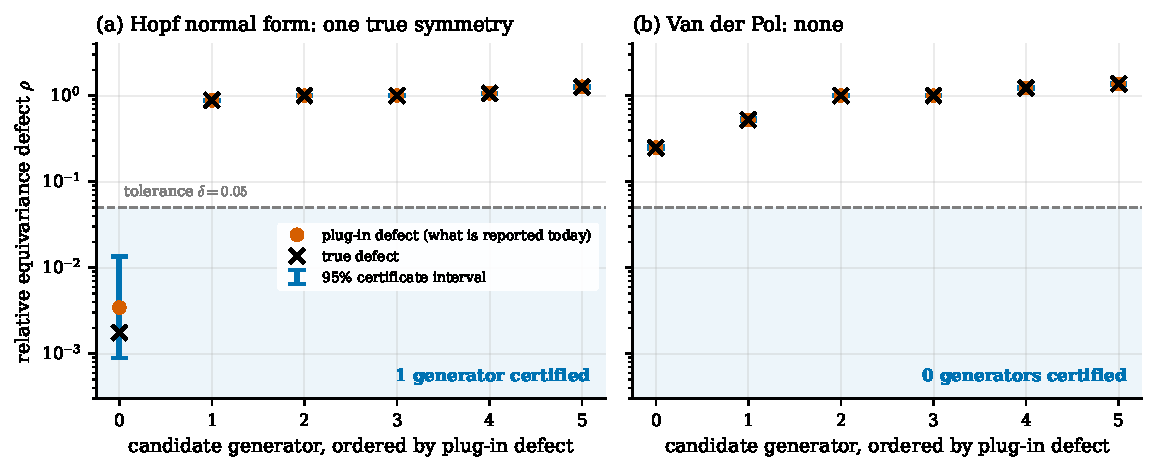
\includegraphics[width=0.82\textwidth]{figures/fig0_example.pdf}
\caption{What the procedure outputs, on two systems at $N = 3200$ and noise
level $0.03$. Each candidate generator gets an interval for its \emph{true}
defect, valid simultaneously across all six. A generator is certified when its
interval lies entirely inside the shaded region below the tolerance. On the
Hopf normal form the rotation generator is certified; on Van der Pol nothing is,
correctly, and the lower certificate goes further, ruling out at $95\%$
confidence the existence of \emph{any} generator in the class with defect below
$0.14$. For the large defects the intervals are narrower than
the plotting symbols: the certificate is only wide where the answer is
genuinely uncertain.}
\label{fig:example}
\end{figure}

\subsection{Two ways to admit model error}
\label{sec:modelerror}

\Cref{prop:simultaneous} is conditional on $\beta^\star$ existing, i.e.\ on
the model class containing the truth. When it does not, we replace $F$ by
$F_\beta + h$ and pay for $h$ explicitly.

\emph{Supremum form.} If $\sup_\Omega \|h\| \le \eta_0$ and
$\sup_\Omega\|Dh\|_F \le \eta_1$ on the target domain, then $[\xi,h]$ moves
the numerator by at most $\eta_1\|\xi\|_{\Ltwo{\nu}} +
\eta_0\|D\xi\|_{\Ltwo{\nu}}$ and each denominator block by at most one of
those terms. Valid for any smooth $h$; conservative, because it spends
supremum norms.

\emph{$L^2$ form.} If the truth lies in a \emph{larger} polynomial class and
the omitted part satisfies $\|h\|_{\Ltwo{\nu}} \le \eta_2$, the numerator
moves by at most $\|B_\theta\|_{\mathrm{op}}\,\eta_2$, where $B_\theta$ is the
exact matrix of $h \mapsto [\xi_\theta, h]$ between the two $\Ltwo{\nu}$
geometries. This is far tighter and is the recommended form. It also makes the
practical advice concrete: \textbf{when in doubt, enlarge the model class}. A
larger class widens the certificate, since more coefficients mean a larger
ellipsoid, but does not invalidate it, whereas a class too small invalidates
it silently.

Both forms are expensive because the Lie derivative \emph{differentiates}: a
model error that is small in size need not be small in slope, and it is the
slope that enters the bracket. A bound stated in $L^2$ therefore has to be
converted into a bound on a derivative, and the conversion constant grows with
the degree of the class the error is allowed to live in. Stating the
model-error assumption directly in a norm that controls one derivative, an
$H^1$ bound, would remove that conversion, and is the obvious refinement; we
do not pursue it here, and we report the cost of not doing so in
\Cref{sec:robustness}.

Neither form can be verified from the data alone, so we treat $\eta$ as a
sensitivity parameter and report the certified tolerance as a function of it,
in the manner standard for unverifiable assumptions elsewhere
\citep{rosenbaum2002observational}. In \Cref{sec:modelclass} we also gate
certification on a lack-of-fit test, which in our experiments detects every
truncated class we tried.

\subsection{What is being assumed}
\label{sec:assumptions}

The value of a certificate is exactly the value of its assumptions.
\begin{enumerate}\itemsep2pt
\item[(A1)] \emph{Model class.} $F = F_{\beta^\star}$ for some $\beta^\star$ in
  the fitted class, or the deviation is bounded as in \Cref{sec:modelerror}.
  This is the binding assumption; \Cref{sec:modelclass} is devoted to it.
\item[(A2)] \emph{Errors.} The observed right-hand sides satisfy
  \eqref{eq:model} with errors independent of the states. Exact validity needs
  Gaussian homoskedastic errors; a sandwich covariance
  \citep{white1980heteroskedasticity} gives asymptotic validity otherwise.
  \Cref{sec:robustness} measures both, and shows where the assumption genuinely fails: when the \emph{states} are noisy and derivatives are differenced, the regressors are noisy and no covariance correction repairs the resulting bias.
\item[(A3)] \emph{Target domain.} The claim is about the user's chosen $\nu$.
  Nothing is asserted outside it. Coverage of $\nu$ by the data enters through
  the design, and \Cref{sec:coverage} quantifies it.
\item[(A4)] \emph{Candidate class.} We find connected subgroups whose generators
  lie in $\mathcal V$. Discrete symmetries are outside this framework, as they
  are outside the Lie-algebraic framework generally.
\end{enumerate}
